\documentclass[conference,a4paper]{IEEEtran}
\IEEEoverridecommandlockouts
\usepackage{cite}
\usepackage{amsmath,amssymb,amsfonts}
\usepackage{graphicx}
\usepackage{booktabs}
\usepackage{multirow}
\usepackage{xcolor}
\usepackage{tikz}
\usetikzlibrary{arrows.meta,positioning,fit,backgrounds}
\usepackage{pgfplots}
\pgfplotsset{compat=1.17}
\usepackage[hidelinks]{hyperref}

\newcommand{\TODO}[1]{\textcolor{red}{[TODO: #1]}}

\begin{document}

\title{Is the VLA Backbone Enough to Read Human Goals?\\ Early Goal Disambiguation from Egocentric Video}

\author{\IEEEauthorblockN{Vu Thi Thu Trang}
\IEEEauthorblockA{\textit{Faculty of \TODO{...}}\\
\textit{VNU University of Engineering and Technology}\\
Hanoi, Vietnam\\
\TODO{email}}
\and
\IEEEauthorblockN{\TODO{Supervisor}}
\IEEEauthorblockA{\textit{Faculty of \TODO{...}}\\
\textit{VNU University of Engineering and Technology}\\
Hanoi, Vietnam\\
\TODO{email}}}

\maketitle

\begin{abstract}
Vision--language--action (VLA) policies such as SmolVLA learn the task goal only from a language instruction. On LIBERO-10, SmolVLA succeeds in 19/100 episodes with the correct instruction and in 0/100 when the instruction is empty. A collaborative robot whose partner does not state the goal therefore needs an \emph{intention module} that reads the goal from what the person does. We build such a module for \emph{early goal disambiguation}: from the first $k\in\{2,4,6,8\}$ frames of an egocentric manipulation step, choose the step's purpose among other purposes from the same video. The study proceeds in stages on 2,503 steps (27 videos, 13 scenes) of EgoIntent, with scene-grouped cross-validation and video-level bootstrap intervals. First, a readout trained on frozen features of SmolVLA's own backbone, SmolVLM2, stays near chance (1.13--1.19$\times$ chance MRR, every interval includes 1). Second, a pretrained SigLIP encoder used without training raises 5-way accuracy to 27.5--28.9\% (chance 20\%). Third, a larger SigLIP encoder combined with subtracting the context of earlier steps in the same video reaches 34.1--38.7\%, and the same configuration is selected in all 8 folds. Fourth, evaluated once on a separate test split, this configuration reaches 30.2\% versus 21.4\% for the base pipeline at $k=8$. Fifth, answering only the most confident half of the queries adds 6.9--7.9 points. Finally, we implement the intention as one extra token in SmolVLA's input and verify the interface with implementation tests.
\end{abstract}

\begin{IEEEkeywords}
intention prediction, egocentric video, vision--language--action models, human--robot collaboration, zero-shot retrieval
\end{IEEEkeywords}

% ---------------------------------------------------------------------
\section{Introduction}
% ---------------------------------------------------------------------

A robot that helps a person at a table is useful only if it acts on the person's goal. Vision--language--action (VLA) models~\cite{brohan2022rt1,zitkovich2023rt2,openx2024,shukor2025smolvla} map camera images, a language instruction and the robot state to motor commands, and the goal reaches them \emph{only} through the instruction. We measure how strong this dependence is: SmolVLA on LIBERO-10 succeeds in 19/100 episodes with the correct instruction and in 0/100 with an empty one. In collaboration, people rarely state every intention, so the robot must infer the goal from what it sees and pass it to the policy in place of the missing instruction.

Inferring the goal from video is hard because early motion is ambiguous, and because the steps of one activity share the same scene and objects. In a dough-kneading video, ``positioning basin'', ``add salt to flour'' and ``forming dough'' all show the same hands, bowl and flour.

This paper asks how to build an intention module for a VLA policy and answers it in stages. Each stage poses one question, and its result motivates the next (Table~\ref{tab:stages}). Our contributions are:
\begin{itemize}
\item \textbf{The VLA backbone does not read human goals.} A readout trained on frozen SmolVLM2 features reaches only 1.13--1.19$\times$ chance MRR on unseen scenes.
\item \textbf{A training-free intention module.} SigLIP so400m with causal subtraction of earlier-step video context reaches \textbf{30.2\%} 5-way accuracy on a test split evaluated once, versus 21.4\% for base SigLIP and 20\% chance. Its confidence margin supports abstention.
\item \textbf{An intention channel for SmolVLA.} We show that SmolVLA fails without goal information (19/100 vs 0/100) and implement a tested interface that injects the intention as one input token.
\end{itemize}

% ---------------------------------------------------------------------
\section{Related Work}
% ---------------------------------------------------------------------

\textbf{Egocentric anticipation and intention.} Large egocentric corpora~\cite{grauman2022ego4d,grauman2024egoexo4d} enabled long-term action anticipation. Intention has been modelled as a latent variable conditioning future actions~\cite{mascaro2023intention}, inferred with large language models~\cite{zhao2024antgpt}, or used to guide reasoning~\cite{chu2026insight}. These works predict future action labels. We isolate a narrower question that matters for assistance: discriminating among \emph{competing purposes} inside one activity from a short prefix. EgoIntent~\cite{egointent2026} provides pre-outcome WHAT/WHY annotations for this.

\textbf{VLA policies.} RT-1/RT-2~\cite{brohan2022rt1,zitkovich2023rt2} and Open X-Embodiment~\cite{openx2024} showed that transformer policies on vision--language features generalise across tasks. SmolVLA~\cite{shukor2025smolvla}, built on LeRobot~\cite{cadene2026lerobot}, couples a 500M SmolVLM2 backbone~\cite{marafioti2025smolvlm} with a flow-matching~\cite{lipman2023flow} action expert. None of these models estimate the intention of a human partner.

\textbf{Image--text alignment.} CLIP~\cite{radford2021clip} and SigLIP~\cite{zhai2023siglip} learn a joint embedding from web-scale image--caption pairs and transfer zero-shot to new label sets. Our results suggest this alignment is what a small-data intention module lacks.

% ---------------------------------------------------------------------
\section{Task, Architecture and Protocol}
% ---------------------------------------------------------------------

\textbf{Task.} Each manipulation step $i$ has a video segment ending before its outcome and a free-form purpose sentence $y_i$ (WHY). Eight frames are sampled uniformly; the module sees only the first $k$. It consists of a video encoder $f$ and a sentence encoder $g$ and scores a candidate sentence $c$ by
\begin{equation}
s(i,c)=\cos\!\big(f(x_{i,1:k}),\,g(c)\big).
\end{equation}
The main metric is \emph{5-way accuracy}: choose $y_i$ among itself and 4 other WHY sentences of the \emph{same video} (chance 20\%). Distractors are fixed per query, so they are identical across all stages. As a secondary metric we rank $y_i$ against all WHY sentences of the held-out fold (several hundred) and report MRR as a multiple of its exact chance level.

\textbf{Architecture.} In VLIA (Fig.~\ref{fig:arch}) the intention module maps the egocentric prefix to an intention vector $\mathbf{z}\in\mathbb{R}^d$. A linear Intention Adapter projects it to the 960-d hidden size of SmolVLA, and the result is inserted as one token after the instruction and before the state token: $[E_{\text{img}};E_{\text{lang}};W\mathbf{z}+b;E_{\text{state}}]$. Because this prefix is cached before the flow-matching steps, the extra token adds negligible cost. Disabling it recovers the original policy exactly.

\begin{figure}[t]
\centering
\resizebox{\columnwidth}{!}{%
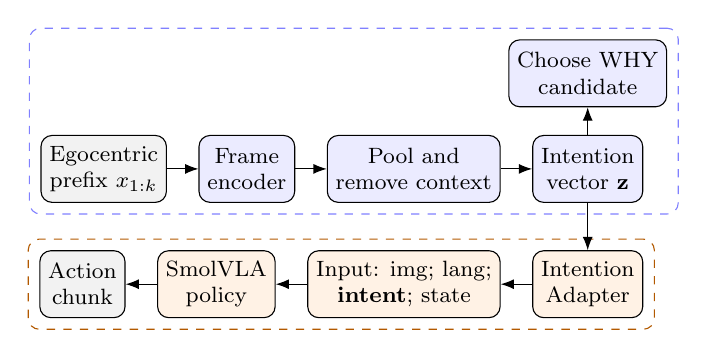
\begin{tikzpicture}[node distance=0.35cm and 0.4cm,
  b/.style={draw,rounded corners,align=center,font=\footnotesize,minimum height=0.85cm,inner sep=3pt},
  >=Latex]
  \node[b,fill=gray!10] (v) {Egocentric\\prefix $x_{1:k}$};
  \node[b,fill=blue!8,right=of v] (e) {Frame\\encoder};
  \node[b,fill=blue!8,right=of e] (p) {Pool and\\remove context};
  \node[b,fill=blue!8,right=of p] (z) {Intention\\vector $\mathbf{z}$};
  \node[b,fill=blue!8,above=0.35cm of z] (c) {Choose WHY\\candidate};
  \draw[->](v)--(e); \draw[->](e)--(p); \draw[->](p)--(z); \draw[->](z)--(c);
  \node[b,fill=orange!10,below=0.6cm of z] (a) {Intention\\Adapter};
  \node[b,fill=orange!10,left=of a] (pre) {Input: img; lang;\\\textbf{intent}; state};
  \node[b,fill=orange!10,left=of pre] (s) {SmolVLA\\policy};
  \node[b,fill=gray!10,left=of s] (act) {Action\\chunk};
  \draw[->](z)--(a); \draw[->](a)--(pre); \draw[->](pre)--(s); \draw[->](s)--(act);
  \begin{scope}[on background layer]
  \node[draw=blue!50,dashed,rounded corners,fit=(v)(e)(p)(z)(c),inner sep=4pt]{};
  \node[draw=orange!70!black,dashed,rounded corners,fit=(a)(pre)(s)(act),inner sep=4pt]{};
  \end{scope}
\end{tikzpicture}}
\caption{VLIA. The intention module (top, Stages 1--5) maps an egocentric prefix to an intention vector; the adapter turns it into one input token of SmolVLA (bottom, Stage 6).}
\label{fig:arch}
\end{figure}

\textbf{Data.} We develop on the train and validation portions of EgoIntent~\cite{egointent2026}, derived from Ego4D: 2,503 steps, 27 videos, 13 scenes (e.g.\ kitchen, workshop, farm), 2,032 distinct WHY sentences.

\textbf{Evaluation.} Scenes are assigned to 8 folds of similar size, and every step is evaluated once, in a scene the model has not seen. Any training or configuration choice uses the training folds only. The EgoIntent test portion (407 steps, 4 videos, after removing one video that overlapped an earlier pilot) is held out and evaluated \emph{once}, for the final configuration. 95\% intervals come from 10,000 bootstrap resamples of whole videos; comparisons use paired per-query differences. Pass/fail criteria, including a practical bar of 30\% 5-way accuracy, were committed to the repository before each stage.

\begin{table}[t]
\caption{Overview of the stages. 5-way: accuracy of choosing the true purpose among 5 same-video candidates (chance 20\%).}
\label{tab:stages}
\centering
\footnotesize
\setlength{\tabcolsep}{3pt}
\begin{tabular}{@{}cp{2.5cm}p{2.6cm}p{2.0cm}@{}}
\toprule
Stage & Question & Result & Next step \\
\midrule
1 & Is the VLA backbone enough? & 1.13--1.19$\times$ chance MRR & Use aligned encoder \\
2 & Does zero-shot alignment help? & 5-way 27.5--28.9\% & Remove shared context \\
3 & Can training-free choices pass 30\%? & 5-way 34.1--38.7\%, same config 8/8 & Freeze, test once \\
4 & Does it hold on unseen videos? & 30.2\% vs 21.4\% ($k=8$) & Add abstention \\
5 & Can it tell when to wait? & $+$6.9--7.9 pts at 50\% coverage & Connect to policy \\
6 & Does SmolVLA need the goal? & 19/100 vs 0/100; interface tested & Replace instruction \\
\bottomrule
\end{tabular}
\end{table}

% ---------------------------------------------------------------------
\section{A Staged Study}
% ---------------------------------------------------------------------

\begin{table}[t]
\caption{Stages 1--2 on scene-held-out folds (2,503 queries). Readout values are means over 3 seeds; brackets are 95\% video-bootstrap intervals. Chance: MRR 0.0298, 5-way 0.20.}
\label{tab:main}
\centering
\setlength{\tabcolsep}{3.5pt}
\footnotesize
\begin{tabular}{llcccc}
\toprule
Encoder & $k$ & MRR & MRR / chance & 5-way & 5-way / chance \\
\midrule
\multirow{4}{*}{\shortstack[l]{Readout\\(MiniLM)}}
 & 2 & .0335 & 1.13 [0.86, 1.43] & .216 & 1.08 [1.00, 1.16] \\
 & 4 & .0345 & 1.16 [0.88, 1.48] & .215 & 1.07 [1.00, 1.16] \\
 & 6 & .0353 & 1.18 [0.90, 1.52] & .212 & 1.06 [0.98, 1.16] \\
 & 8 & .0347 & 1.17 [0.87, 1.51] & .219 & 1.10 [1.01, 1.20] \\
\midrule
\multirow{4}{*}{\shortstack[l]{Readout\\(SmolVLM2)}}
 & 2 & .0340 & 1.14 [0.95, 1.36] & .219 & 1.09 [1.02, 1.17] \\
 & 4 & .0338 & 1.14 [0.94, 1.35] & .222 & 1.11 [1.03, 1.19] \\
 & 6 & .0346 & 1.16 [0.95, 1.39] & .223 & 1.12 [1.04, 1.20] \\
 & 8 & .0354 & 1.19 [0.98, 1.42] & .230 & 1.15 [1.07, 1.23] \\
\midrule
\multirow{4}{*}{\shortstack[l]{Base SigLIP\\zero-shot}}
 & 2 & .0671 & 2.25 [1.87, 2.75] & .277 & 1.39 [1.23, 1.56] \\
 & 4 & .0715 & 2.40 [2.02, 2.88] & .275 & 1.38 [1.22, 1.55] \\
 & 6 & .0734 & 2.47 [2.06, 2.97] & .281 & 1.40 [1.24, 1.58] \\
 & 8 & .0765 & 2.57 [2.13, 3.14] & .289 & 1.44 [1.27, 1.62] \\
\bottomrule
\end{tabular}
\end{table}

\subsection{Stage 1: a readout on the VLA backbone}
\textbf{Method.} Each frame is encoded by frozen SmolVLM2-500M-Video-Instruct (960-d); the first $k$ vectors are mean-pooled and passed through a two-layer MLP (512 hidden units). Targets are a frozen sentence encoder (all-MiniLM-L6-v2~\cite{reimers2019sbert}) or SmolVLM2 text features reduced to 256-d by PCA. Training uses multi-positive InfoNCE ($\tau=0.07$) plus $0.1\times$ a cosine loss, AdamW (lr $10^{-3}$), up to 100 epochs chosen on an inner split of the training scenes, three seeds. Mean pooling is the starting point because, in a pilot on a small split, structured WHAT$\to$WHY models did not beat it.

\textbf{Result.} The readout is close to chance (Table~\ref{tab:main}): MRR is 1.13--1.19$\times$ chance and every interval includes 1; 5-way accuracy is 21.9--23.0\% with SmolVLM2 targets. On the original fixed split, validation MRR had looked like 1.7--1.9$\times$ chance, but with epochs selected on that same split; on the held-out test portion the readout's best MRR (0.0314) equals chance (0.0318). Letting SmolVLM2 score each candidate by its own likelihood (no training) gives 23.5--24.6\% 5-way accuracy, above chance but still weak. \emph{The VLA backbone carries little usable goal signal at this data scale}, which leads to Stage 2.

\subsection{Stage 2: zero-shot image--text alignment}
\textbf{Method.} We encode frames with the image tower of \texttt{siglip-base-patch16-224}~\cite{zhai2023siglip} (``base SigLIP''), mean-pool the first $k$, and encode candidates with the text tower. Nothing is trained.

\textbf{Result.} With no trained parameters, base SigLIP reaches 2.25--2.57$\times$ chance MRR; its interval lower bounds (1.87--2.13) lie above the readout's upper bounds at every $k$. 5-way accuracy is 27.5--28.9\%, below the 30\% bar. More frames help: from 2 to 8 frames MRR rises by $+0.0094$ [$+0.0053$, $+0.0141$] and 5-way accuracy by $+1.1$ points [$+0.1$, $+2.1$], whereas the readout's gains have intervals containing 0. The typical error recognises the activity but not the step: for ``positioning basin'', base SigLIP prefers ``prepare to knead dough'' and ``forming cohesive dough''. Every frame of the video shows the same table, bowl and hands, and this shared content dominates the embedding. Stage 3 removes it.

\subsection{Stage 3: training-free configuration selection}
\textbf{Method.} We search 90 training-free configurations: 5 encoders (SigLIP base 224/384, SigLIP2 base, SigLIP so400m, CLIP ViT-L/14) $\times$ 3 frame aggregations (mean; max of per-frame cosine; log-sum-exp) $\times$ 3 embedding corrections $\times$ 2 text templates (raw WHY; ``a first-person photo of a person doing: \{why\}''). The corrections are none, subtracting a global training mean, and \emph{context removal}: subtracting the mean embedding of all frames of \emph{strictly earlier} steps of the same video, which keeps what is new in the current step and stays causal (the first step of a video, 1\% of queries, falls back to the global mean). To avoid optimistic selection, each outer fold picks the configuration with the best 5-way accuracy on its \emph{training} folds only and applies it to the held-out fold.

\textbf{Result.} All 8 folds pick the same configuration, \emph{SigLIP so400m, mean pooling, context removal, template}; we call it the \emph{proposed pipeline}. 5-way accuracy rises to 34.1--38.7\%, with paired gains of $+6.4$ to $+9.9$ points over base SigLIP, all intervals above 0 (Table~\ref{tab:ladder}). The MRR gain is positive but its intervals contain 0. Replacing frames by those of a video from another scene ($k=8$, 313 queries) drops accuracy from 39.6\% to 18.8\%, so the signal comes from the video. Both parts matter: so400m without context removal gives 31.1--33.0\%, base SigLIP with it 29.1--32.1\%. The configuration was then frozen into a hashed file before the test portion was read.

\begin{table}[t]
\caption{5-way accuracy of base SigLIP (B) and the proposed pipeline (P). CV: out-of-fold, 2,503 queries. Test: held-out split, 407 queries, 4 videos, evaluated once. $\Delta$: paired P$-$B in points, 95\% video-bootstrap interval.}
\label{tab:ladder}
\centering
\setlength{\tabcolsep}{2.6pt}
\footnotesize
\begin{tabular}{ccccccc}
\toprule
& \multicolumn{3}{c}{Cross-validation (Stage 3)} & \multicolumn{3}{c}{Test, run once (Stage 4)} \\
\cmidrule(lr){2-4}\cmidrule(lr){5-7}
$k$ & B & P & $\Delta$ & B & P & $\Delta$ \\
\midrule
2 & 27.7 & 34.1 & +6.4 [3.9, 8.9] & 20.4 & 21.9 & +1.5 [$-$1.0, 3.8] \\
4 & 27.5 & 34.9 & +7.4 [4.9, 10.0] & 21.1 & 24.6 & +3.4 [1.3, 4.8] \\
6 & 28.1 & 36.2 & +8.2 [5.1, 11.2] & 22.4 & 27.8 & +5.4 [1.0, 9.7] \\
8 & 28.9 & 38.7 & +9.9 [6.2, 13.4] & 21.4 & 30.2 & +8.9 [4.4, 14.8] \\
\bottomrule
\end{tabular}
\end{table}

\subsection{Stage 4: one evaluation on unseen videos}
On the 407 held-out steps, the proposed pipeline is above chance at all four $k$ and above base SigLIP at $k=4,6,8$, reaching 30.2\% versus 21.4\% at $k=8$ (Table~\ref{tab:ladder}). Swapping in another scene's frames drops it from 31.4\% to 21.6\%. Absolute accuracy is lower than in cross-validation, and base SigLIP drops too, so the test videos appear harder; with only 4 videos the intervals rest on 4 clusters. Gallery MRR of the proposed pipeline is \emph{below} base SigLIP at every $k$: context removal separates steps within a video, which is the assistance-relevant case, but discards the scene cue that helps ranking across videos.

\subsection{Stage 5: knowing when to wait}
Using the top-1 minus top-2 margin as confidence, with thresholds set from the other folds, answering the 50\% most confident queries raises accuracy by $+6.9$ to $+7.9$ points (lower bounds $\geq 3.9$), and answering 20\% reaches 53--61\%. On base SigLIP the gain is only 2.6--3.5 points. Three other ideas did not help: stopping observation at the first confident frame did not beat a fixed $k$ at matched frame budgets; mixing in WHY sentences of the nearest training queries lowered MRR; and a hand-region variant was not run because MediaPipe~\cite{zhang2020mediapipe} detected hands in only 58.2\% of frames (below 30\% in four scenes).

\subsection{Stage 6: connecting intention to SmolVLA}
\textbf{Does SmolVLA need the goal?} A SmolVLA checkpoint retrained on LIBERO-10~\cite{liu2023libero} (7-D actions, 25k steps) is run on 10 tasks $\times$ 10 episodes with the correct instruction, an empty one, and another task's instruction; episode $e$ uses the same initial state and seed in every condition. It succeeds in 19/100 episodes with the correct instruction (Wilson [12.5, 27.8]\%) and in 0/100 in both other conditions (both [0, 3.7]\%); every failed episode runs to the 520-step limit.

\textbf{Interface.} With 256-, 768- and 1152-d intention vectors, the adapter receives gradients, the input grows by exactly one token placed before the state token, the token is present in the KV cache, the flow-matching loss is finite, checkpoints round-trip, and disabling the token reproduces the original SmolVLA. These tests establish correctness, not a behavioural benefit.

% ---------------------------------------------------------------------
\section{Discussion and Limitations}
% ---------------------------------------------------------------------

The main lesson is a design one: with about two thousand labelled steps, an intention module cannot learn the visual--linguistic mapping from the VLA backbone's features, while a pretrained aligned encoder provides it for free. Removing the context of earlier steps is a cheap, causal addition that helps exactly in the within-activity setting a collaborative robot faces. The limitations are substantial. The study covers 27 videos in 13 scenes. The test split has only 4 videos, is not scene-disjoint, and shows a clear drop from cross-validation. Context removal lowers cross-video ranking. WHY sentences are free-form and 44.5\% of queries have a near-paraphrase in the same video, which caps exact-match scores. The LIBERO ablation uses one checkpoint and 10 episodes per task, and a predicted intention has not yet been used to drive the policy.

% ---------------------------------------------------------------------
\section{Conclusion and Next Step}
% ---------------------------------------------------------------------

A readout on the VLA's frozen backbone is near chance at reading human goals, whereas a training-free image--text pipeline with causal context removal reaches 34--39\% 5-way accuracy in cross-validation and 30.2\% on a test split evaluated once, with a usable confidence signal. Since SmolVLA fails without goal information, the next step is to train it with an always-empty instruction so that the goal reaches the policy only through the intention token, and to compare the correct intention against an empty instruction and against another task's intention. Code and result files are at \url{https://github.com/sgdfgnhmjnfd/vlia-uet}.

\begin{thebibliography}{99}
\bibitem{brohan2022rt1} A.~Brohan \emph{et al.}, ``RT-1: Robotics transformer for real-world control at scale,'' arXiv:2212.06817, 2022.
\bibitem{zitkovich2023rt2} B.~Zitkovich \emph{et al.}, ``RT-2: Vision-language-action models transfer web knowledge to robotic control,'' in \emph{Proc. CoRL}, 2023, pp.~2165--2183.
\bibitem{openx2024} Open X-Embodiment Collaboration, ``Open X-Embodiment: Robotic learning datasets and RT-X models,'' in \emph{Proc. ICRA}, 2024, pp.~6892--6903.
\bibitem{shukor2025smolvla} M.~Shukor \emph{et al.}, ``SmolVLA: A vision-language-action model for affordable and efficient robotics,'' arXiv:2506.01844, 2025.
\bibitem{cadene2026lerobot} R.~Cadene \emph{et al.}, ``LeRobot: An open-source library for end-to-end robot learning,'' in \emph{Proc. ICLR}, 2026.
\bibitem{marafioti2025smolvlm} A.~Marafioti \emph{et al.}, ``SmolVLM: Redefining small and efficient multimodal models,'' arXiv:2504.05299, 2025.
\bibitem{lipman2023flow} Y.~Lipman, R.~T.~Q. Chen, H.~Ben-Hamu, M.~Nickel, and M.~Le, ``Flow matching for generative modeling,'' in \emph{Proc. ICLR}, 2023.
\bibitem{grauman2022ego4d} K.~Grauman \emph{et al.}, ``Ego4D: Around the world in 3,000 hours of egocentric video,'' in \emph{Proc. CVPR}, 2022, pp.~18995--19012.
\bibitem{grauman2024egoexo4d} K.~Grauman \emph{et al.}, ``Ego-Exo4D: Understanding skilled human activity from first- and third-person perspectives,'' in \emph{Proc. CVPR}, 2024, pp.~19383--19400.
\bibitem{mascaro2023intention} E.~Valls Mascaro, H.~Ahn, and D.~Lee, ``Intention-conditioned long-term human egocentric action anticipation,'' in \emph{Proc. WACV}, 2023, pp.~6048--6057.
\bibitem{zhao2024antgpt} Q.~Zhao \emph{et al.}, ``AntGPT: Can large language models help long-term action anticipation from videos?'' in \emph{Proc. ICLR}, 2024.
\bibitem{chu2026insight} Q.~Chu, H.~Zhang, M.~Liu, Y.~Feng, H.~Shi, and L.~Nie, ``Intention-guided cognitive reasoning for egocentric long-term action anticipation,'' in \emph{Proc. AAAI}, 2026.
\bibitem{egointent2026} ``EgoIntent: An open-ended benchmark for intent understanding at pre-outcome micro-steps in egocentric procedural activities,'' Hugging Face dataset \texttt{py2279105943/EgoIntent}, 2026.
\bibitem{radford2021clip} A.~Radford \emph{et al.}, ``Learning transferable visual models from natural language supervision,'' in \emph{Proc. ICML}, 2021, pp.~8748--8763.
\bibitem{zhai2023siglip} X.~Zhai, B.~Mustafa, A.~Kolesnikov, and L.~Beyer, ``Sigmoid loss for language image pre-training,'' in \emph{Proc. ICCV}, 2023, pp.~11975--11986.
\bibitem{reimers2019sbert} N.~Reimers and I.~Gurevych, ``Sentence-BERT: Sentence embeddings using Siamese BERT-networks,'' in \emph{Proc. EMNLP-IJCNLP}, 2019, pp.~3982--3992.
\bibitem{zhang2020mediapipe} F.~Zhang \emph{et al.}, ``MediaPipe Hands: On-device real-time hand tracking,'' arXiv:2006.10214, 2020.
\bibitem{liu2023libero} B.~Liu, Y.~Zhu, C.~Gao, Y.~Feng, Q.~Liu, Y.~Zhu, and P.~Stone, ``LIBERO: Benchmarking knowledge transfer for lifelong robot learning,'' in \emph{Proc. NeurIPS}, 2023.
\end{thebibliography}

\end{document}
